\documentclass[12pt]{article}

\usepackage{enumerate}
\usepackage{amsmath}
\usepackage{amsthm}
\usepackage{amssymb}
\usepackage{changepage}
\usepackage{graphicx}
\usepackage[a4paper, margin=1in]{geometry}
\allowdisplaybreaks[1]

\title{DATA315 Assignment 1}
\author{Rin Meng 51940633}
\date{\today}

\begin{document}

\maketitle

\begin{enumerate}
    \item Suppose $Y = 3X + Z$ where $Z$ and $X$ are independent random variables. Suppose $X$
    has mean 5 and variance 1 and Z has mean 0 and variance 9.
    \begin{enumerate} 
        \item $E[Y] = E[3Y + Z] = E[3Y] + E[Z] = 3E[Y] + E[Z] = 3 \cdot 5 + 0 = 15$
        \item $V(2X) = 2^2V(X) = 4 \cdot 1$
        \item $E[X^2] = V(X) + E[X]^2 = 1 + 5^2 = 26$
        \item $E[XY] = E[3X^2 + XZ] = 3E[X^2] + E[XZ] = 3 \cdot 26 + 0 = 78$
        \item $Cov(X, Y) = E[XY] - E[X]E[Y] = 78 - 5 \cdot 15 = 3$
        \item $E[Y | Z = 2] = E[3X + 2 | Z = 2] = 3E[X | Z = 2] + 2 = 3 \cdot 5 + 2 = 17$
    \end{enumerate}
    \item Suppose $X$ is a normal random variable with mean 2.0 and standard deviation
    0.8, and suppose $Y = 5X + 7$. Find the mean and standard deviation of $Y$.
    \begin{enumerate}
        \item $E[Y] = E[5X + 7] = 5E[X] + 7 = 5 \cdot 2 + 7 = 17$
        \item $V(Y) = V(5X + 7) = 5^2V(X) = 5^2 \cdot 0.8$
        \item $SD(Y)^2 = V(Y) \Rightarrow SD(Y) = \sqrt{V(Y)} = \sqrt{5^2 \cdot 0.8} = 2\sqrt{5}$
    \end{enumerate}
    \item Calculate the sample average and sample standard deviation of the level
    observations in \verb|LakeHuron|. Use R for this question and submit the code together with
    your answers.
    \begin{verbatim}
> data(LakeHuron)
> sample_average <- mean(LakeHuron)
> sample_sd <- sd(LakeHuron)
> print(paste("Sample Average:", sample_average))
[1] "Sample Average: 579.004081632653"
> print(paste("Sample Standard Deviation:", sample_sd))
[1] "Sample Standard Deviation: 1.31829852597076"
    \end{verbatim}
    \item  Suppose $Z1, Z2 \text{ and } Z3$ are independent standard normal random variables.
    Write down the joint pdf for $Z1, Z2 \text{ and } Z3$.
    \begin{align*}
        f(z_1, z_2, z_3) &= f(z_1) f(z_2) f(z_3) \\
        &= \frac{1}{\sqrt{2\pi}} e^{-\frac{z_1^2}{2}} \cdot \frac{1}{\sqrt{2\pi}} e^{-\frac{z_2^2}{2}} \cdot \frac{1}{\sqrt{2\pi}} e^{-\frac{z_3^2}{2}} \\
        &= \frac{1}{(2\pi)^{3/2}} e^{-\frac{z_1^2 + z_2^2 + z_3^2}{2}}
    \end{align*}
    \item  Suppose $Z1, Z2, \ldots , Zn$ are time series with white noise model
    \[ z_t = \varepsilon_t \]
    where $\varepsilon_t$ is independent random variable with exponiential distribution $exp(\lambda)$.
    Find the maximum likelihood estimator for $\lambda$.
    \begin{align*}
        f(z_t) &= \lambda e^{-\lambda z_t} \\
        L(\lambda) &= \prod_{t=1}^{n} f(z_t) \\
        &= \prod_{t=1}^{n} \lambda e^{-\lambda z_t} \\
        &= \lambda^n e^{-\lambda \sum_{t=1}^{n} z_t} \\
        \log L(\lambda) &= n \log \lambda - \lambda \sum_{t=1}^{n} z_t \\
        \frac{d}{d\lambda} \log L(\lambda) &= \frac{n}{\lambda} - \sum_{t=1}^{n} z_t \\
        \frac{n}{\lambda} - \sum_{t=1}^{n} z_t &= 0 \\
        \hat{\lambda} &= \frac{n}{\sum_{t=1}^{n} z_t} \\
        \because \bar{z} &= \frac{1}{n} \sum_{t=1}^{n} z_t \\
        \hat{\lambda} &= \frac{n}{n \bar{z}} = \frac{1}{\bar{z}}
    \end{align*}
    \item Suppose $Z_1, Z_2, \ldots, Z_n$ is a time series. Let 
    \[ L(\rho) \sum_{t = 2}^{n}(Z_t - \rho Z_{t-1})^2 \]
    \begin{enumerate}
        \item  Using calculus, find a formula for $\hat{\rho}$, the value of $\rho$ 
        which minimizes $L(\rho)$. (This is the least-squares estimator for $\rho$, 
        the so-called lag 1 autocorrelation.)
        \begin{align*}
            \frac{d}{d\rho} L(\rho) &= \frac{d}{d\rho} \sum_{t = 2}^{n}(Z_t - \rho Z_{t-1})^2 \\
            &= \sum_{t = 2}^{n} 2(Z_t - \rho Z_{t-1}) \cdot (-Z_{t-1}) \\
            &= -2 \sum_{t = 2}^{n} Z_{t-1} Z_t + 2 \rho \sum_{t = 2}^{n} Z_{t-1}^2 \\
            &= 0 \\
            \sum_{t = 2}^{n} Z_{t-1} Z_t &= \rho \sum_{t = 2}^{n} Z_{t-1}^2 \\
            \hat{\rho} &= \frac{\sum_{t = 2}^{n} Z_{t-1} Z_t}{\sum_{t = 2}^{n} Z_{t-1}^2}
        \end{align*}
        \item Suppose, in addition, that \( Z_1, Z_2, \ldots, Z_n \) are independent normally distributed random variables with mean 0 and standard deviation \( \sigma \).
            Find $E\left[\sum_{t=2}^n Z_t Z_{t-1}\right]$ and $E\left[\sum_{t=1}^{n-1} Z_t^2\right]$.
            \begin{enumerate}
                \item 
                \begin{align*}
                    E\left[\sum_{t=2}^n Z_t Z_{t-1}\right] &= \sum_{t=2}^n E[Z_t Z_{t-1}] \\
                    &= \sum_{t=2}^n E[Z_t] E[Z_{t-1}] \\
                    &= \sum_{t=2}^n 0 \cdot 0 \\
                    &= 0
                \end{align*}
                \item 
                \begin{align*}
                    E\left[\sum_{t=1}^{n-1} Z_t^2\right] &= \sum_{t=1}^{n-1} E[Z_t^2] \\
                    &= \sum_{t=1}^{n-1} \text{Var}(Z_t) \\
                    &= \sum_{t=1}^{n-1} \sigma^2 \\
                    &= (n-1) \sigma^2
                \end{align*}
            \end{enumerate} 
        \item 
            Let  
            \[ X_t = Z_{t-1}, \quad t = 2, \ldots, n \]  
            and  
            \[ Y_t = Z_t, \quad t = 1, \ldots, n-1. \]  
            Write down the formula for the sample correlation between \( X \) and \( Y \),
            expressed in terms of the \( Z \)'s, and compare the formula you obtained with 
            \( \hat{\rho} \) obtained in part (a).
            \begin{align*}
                \hat{\rho}_{XY} &= \frac{\text{Cov}(X, Y)}{\sqrt{\text{Var}(X) \text{Var}(Y)}} \\
                \text{Cov}(X, Y) &= \frac{1}{n-1} \sum_{t=1}^{n-1} (X_t - \bar{X})(Y_t - \bar{Y}) \\
                &\Rightarrow \sum_{t=1}^{n-1} (Z_{t-1} - \bar{Z}_{t-1})(Z_t - \bar{Z}_t) \\
                \text{Var}(X) &= \frac{1}{n-1} \sum_{t=1}^{n-1} (X_t - \bar{X})^2 \\
                &\Rightarrow \frac{1}{n-1} \sum_{t=1}^{n-1} (Z_{t-1} - \bar{X})^2 \\
                \text{Var}(Y) &= \frac{1}{n-1} \sum_{t=1}^{n-1} (Y_t - \bar{Y})^2 \\
                &\Rightarrow \frac{1}{n-1} \sum_{t=1}^{n-1} (Z_t - \bar{Y})^2 \\
                \bar{X} &= \frac{1}{n-1} \sum_{t=1}^{n-1} Z_{t-1} \\
                \bar{Y} &= \frac{1}{n-1} \sum_{t=1}^{n-1} Z_t \\
                \hat{\rho}_{XY} &= \frac{\sum_{t=1}^{n-1} (Z_{t-1} - \bar{Z}_{t-1})(Z_t - \bar{Z}_t)}{\sqrt{\sum_{t=1}^{n-1} (Z_{t-1} - \bar{Z}_{t-1})^2 \sum_{t=1}^{n-1} (Z_t - \bar{Z}_t)^2}} \\
                \hat{\rho}_{XY} &= \frac{\sum_{t = 2}^{n} (Z_{t-1} - \bar{X})(Z_t - \bar{Y})}{\sqrt{\sum_{t = 2}^{n} (Z_{t-1} - \bar{X})^2 \sum_{t = 2}^{n} (Z_t - \bar{Y})^2}} \\
            \end{align*}
            If $\hat{\rho}$ from part (a) is the sample autocorrelation of $Z$ then at lag 1, then:
            \[ \hat{\rho} = \frac{\sum_{t = 2}^{n} Z_{t-1} Z_t}{\sum_{t = 2}^{n} Z_{t-1}^2} \]
            The formula for $\hat{\rho}_{XY}$ is similar but includes centering with the sample means,
                $\bar{X}$ and $\bar{Y}$. If $Z_t$ has mean of 0, then $\bar{X} = \bar{Y} = 0$ 
            then it is true that $\hat{\rho} = \hat{\rho}_{XY}$.
            \[ \hat{\rho}_{XY} = \frac{\sum_{t = 2}^{n} Z_{t-1} Z_t}{\sqrt{\sum_{t = 2}^{n} Z_{t-1}^2 \sum_{t = 2}^{n} Z_t^2}} \]
            \[ \hat{\rho}_{XY} = \frac{\sum_{t = 2}^{n} Z_{t-1} Z_t}{\sum_{t = 2}^{n} Z_{t-1}^2} \]
    \end{enumerate}
    \item 
        Let \( Z_t \) be the time series where \( t = 1, 2, \ldots, n \). Consider a time series with \( n = 4 \).

        \begin{enumerate}
            \item Find the distribution of the statistic \( \tau \) for the Mann-Kendall test.
            Since it is a time series wiht $n = 4$, then we would have
            
            
            \item Verify in these cases that the variance of \( \tau \) is \( \frac{2(2n+5)9}{n(n-1)} \).
            \item Suppose \( z_1, z_2, z_3, z_4 \) are \( 0.2, 0.25, 0.22, 0.3 \). Perform the Mann-Kendall test using the exact distribution you have derived.
        \end{enumerate}
        
    \item The data in \verb|DAAG::vlt$prize| consist of a time series of observations of prize
        winnings (in dollars) taken on a video lottery terminal in a sequence of 345 plays. Obtain
        a trace plot of the series and conduct a trend test. Is there strong evidence of a decrease
        or increase in the prize winnings over time?
    \begin{verbatim}
> library(DAAG)
> library(ggplot2)
> data(vlt)
> prize <- vlt$prize
> ggplot(data = data.frame(play = 1:345, 
prize = prize), aes(x = play, y = prize)) +
geom_line() + labs(x = "Play number", 
y = "Prize (dollars)", 
title = "Trace Plot of Prize Winnings")
    \end{verbatim}
    \begin{center}
        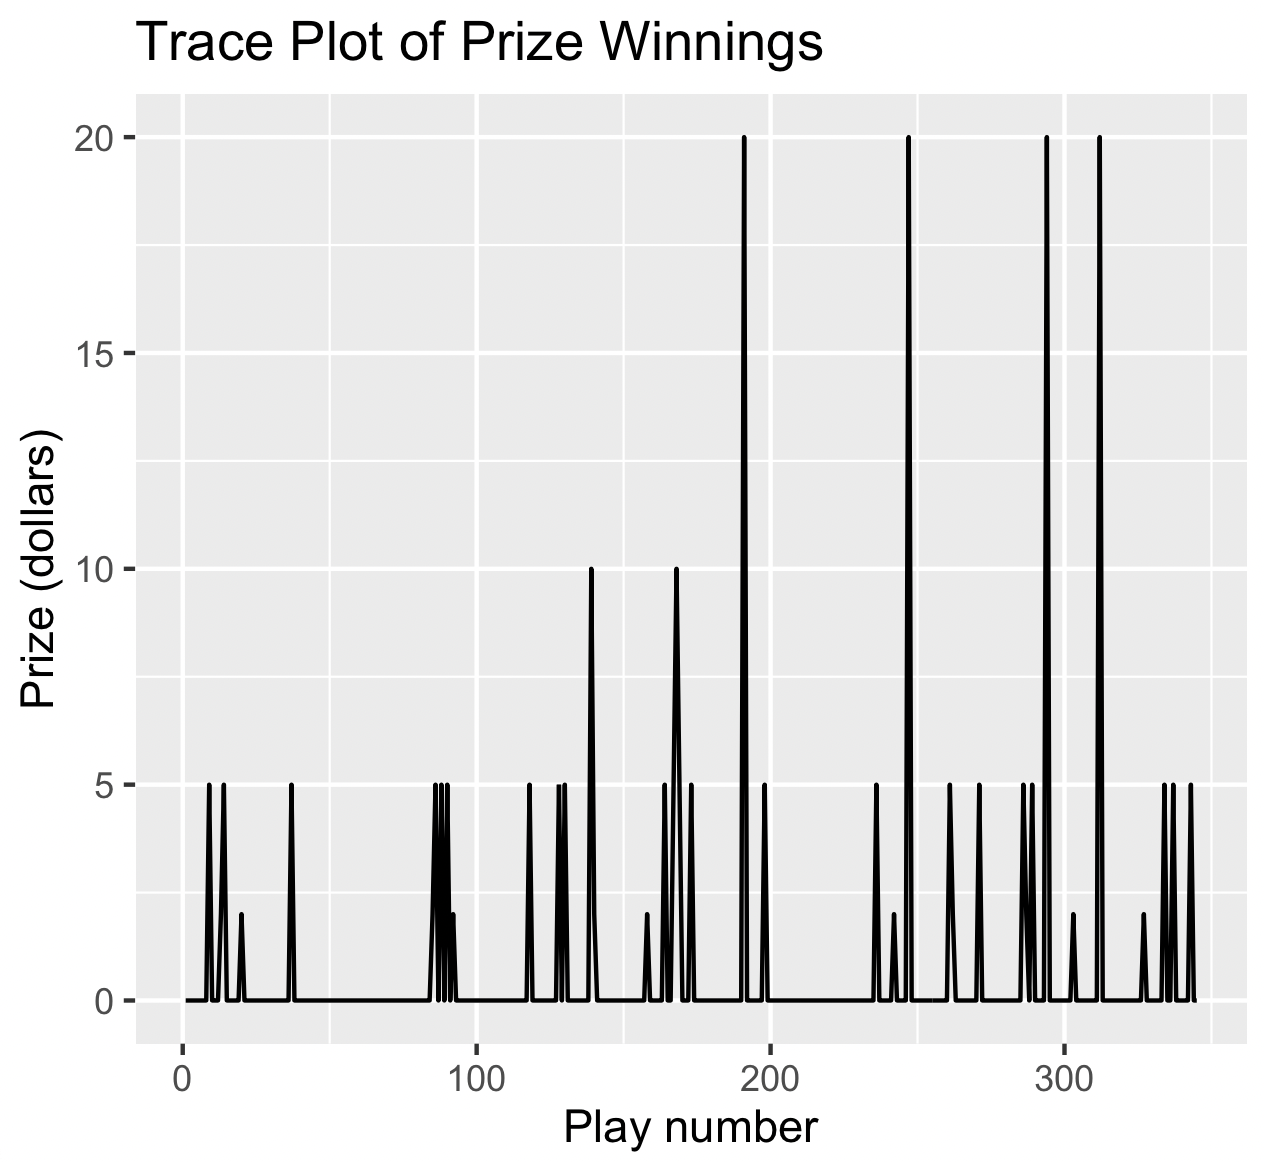
\includegraphics[width=0.8\textwidth]{traceplot.png}
    \end{center}
    Here, we can see that there is a random fluctuations in the prize winnings over time. 
    Now we use the Mann-Kendall test, to test for a trend.
    \begin{verbatim}
> library(Kendall)
> MannKendall(prize)
tau = 0.0367, 2-sided pvalue = 0.3973
    \end{verbatim}
    This suggests that there is an upward trend, but the p-value 
    is not significant enough to reject the null hypothesis that there is no trend.
    $\therefore$ There is no evidence of a systematic increase or decrease in prize winnings over the 345 plays.
    \item Consider the time series: $13, 11, 14, 17, 16, 15$.
    Conduct the Mann-Kendall trend test by hand, using the following steps.
    \begin{enumerate}
        \item Calculate the value of $\tau$ showing the steps that you are using.
        
        \item Calculate the variance of $\tau$ under the null hypothesis.
        
        \item Under the approximate normal assumption, calculate the test statistic using \(\tau\) and the standard error. 
        What would you conclude from this test?
        
    \end{enumerate}
\end{enumerate}

\end{document}
